% datum?
\documentclass[thesis=B,czech,hidelinks]{FITthesis}[2019/03/06]

% my packages and stuff
\usepackage{todonotes}
\usepackage{xevlna}
% from https://tex.stackexchange.com/a/251025
\usepackage{relsize}
\usepackage{xspace}
\newcommand{\Rplus}{\protect\hspace{-.1em}\protect\raisebox{.35ex}{\smaller{\smaller\textbf{+}}}}
\newcommand{\Cpp}{\mbox{C\Rplus\Rplus}\xspace}
\usepackage[backend=biber,style=iso-numeric,sortlocale=cs_CZ,autolang=other,bibencoding=UTF8]{biblatex}
\usepackage[outputdir=build]{minted}
\renewcommand{\listingscaption}{Ukázka zdrojového kódu} %místo Listing ve výpisu bude Výpis kódu
\renewcommand{\listoflistingscaption}{Seznam ukázek zdrojového kódu} %místo List of Listings vypíšeme Seznam výpisů kódu
\counterwithin{listing}{chapter} %číslování prostředí listing v rámci kapitol

\addbibresource{mybibliographyfile.bib}

\hyphenation{NETCONF NETCONFu knihovnu knihovny}


\department{Katedra softwarového inženýrství}
\title{Nástroj pro konfiguraci a monitorování}
\authorGN{Václav}
\authorFN{Kubernát}
\authorWithDegrees{Václav Kubernát}
\author{Václav Kubernát}
\supervisor{Ing. Tomáš Čejka, Ph.D.}
% TODO: dopsat
\acknowledgements{Doplňte, máte-li komu a za co děkovat. V~opačném případě úplně odstraňte tento příkaz.}

\abstractCS{Tato práce se zabývá vytvořením interaktivní konzolové aplikace sloužící ke konfiguraci síťových zařízení pomocí protokolu \textit{NETCONF}. Tento program slouží jako alternativa k dostupným, méně intuitivním, řešením. Toho dosahuje přívětivým uživatelským rozhraním implementovaným pomocí kniho\-vny \textit{replxx}.

Řešení využívá generátorů parserů, které jsou definovány deklarativně, knihovnu \textit{libyang} pro manipulaci s modelovacím jazykem \textit{YANG} a \textit{libnetconf} pro komunikaci přes protokol \textit{NETCONF}.
}

\abstractEN{This thesis focuses on creating an interactive console application with the purpose of configuring network devices over the \textit{NETCONF} protocol. This program serves as an alternative to available, but less intuitive solutions. This is achieved mainly by creating a user-friendly interface implemented by the \textit{replxx} library.

The solution uses \textit{Boost Spirit X3} to create parsers defined declaratively, \textit{libyang} library for manipulating the \textit{YANG} modeling language, and \textit{\mbox{libnetconf}} for communication over \textit{NETCONF}.
}
\placeForDeclarationOfAuthenticity{V~Praze}
% TODO: zkontrolovat
\declarationOfAuthenticityOption{4} %volba Prohlášení (číslo 1-6)

\keywordsCS{netconf, yang, síťová konfigurace, konfigurace, cli, interaktivní cli, parsování}
\keywordsEN{netconf, yang, network configuration, configuration, cli, interactive cli, parsing}

\begin{document}

\begin{introduction}
Ke konfiguraci síťových zařízení existuje mnoho nástrojů. Pro klasického uživatele je nejlepší volba nějakého grafického rozhraní, ve kterém lze nastavit esenciální funkce jako například název nebo zabezpečení bezdrátové sítě. Pro síťové administrátory, kteří musí spravovat mnoho síťových zařízení najednou, je ovšem takové řešení nevhodné, protože jej nelze používat v různých administrátorských skriptech apod. V těchto případech je tedy nutné použít nějakou konzolovou aplikaci. V této práci implementuji program, který umožní administrátorům jednoduše a intuitivně konfigurovat síťová zařízení.

Pokud chceme konfigurovat zařízení po síti, je třeba nejprve způsob komunikace se zařízeními standardizovat. \textit{NETCONF}\,\cite{rfcNetconf} byl vytvořen organizací IETF\footnote{Internet Engineering Task Force; organizace zabývající se vývojem internetových standardů} jako standard pro konfiguraci síťových zařízení. \textit{NETCONF} neřeší způsob reprezentace konfiguračních dat, a proto byl pro tyto potřeby vytvořen modelovací jazyk \textit{YANG}\,\cite{rfcYang}. Moje aplikace komunikuje s zařízeními právě pomocí těchto dvou standardů. Více o těchto standardech píši v teoretické části práce.

V návrhové části práce se věnuji tomu, jakým způsobem lze program používat a rozebírám syntaxi programu. Aplikace by měla být intuitivní, což znamená že by ji uživatel měl být schopný ovládat i bez detailní znalosti \textit{NETCONFu} nebo konkrétních modelů \textit{YANG}. Prostředky pro tuto \uv{intuitivnost} jsou zde popsány též.

Hlavním důvodem výběru této bakalářské práce je především použití generátoru parserů \textit{Boost Spirit X3}. Aplikace využívá tuto knihovnu k realizaci syntaxe, pomocí které je program ovládán. O \textit{Spiritu} a dalších prostředcích, které moje aplikace využívá se píši v implementační části práce.
\end{introduction}

\chapter{Teoretická část}
V rámci práce se věnuji různým klíčovým technologiím a pojmům. V této kapitole vysvětluji použité standardy a teorii formálních jazyků, která mi pomáhá s vytvářením parserů.


\section{YANG}
\textit{YANG} je jazyk sloužící k modelování konfigurace. Pomocí různých zabudovaných konstruktů lze vybudovat konfigurační strom, který logicky sdružuje různé druhy konfigurace, definuje, kde lze jakou hodnotu nastavit, jaké mají hodnoty datové typy apod. Kromě konfigurace podporuje \textit{YANG} i definování různých procedur. Kódování dat funguje pomocí XML\footnote{Extensible Markup Language; značkovací jazyk sloužící především k ukládání a přenosu dat}\@.

\textit{YANG} definuje konfigurační modely pomocí tzv. \textit{modulů}. Modul je nejvrchnější složkou konfigurace a vše ostatní se definuje v něm. \textit{YANG} podporuje mnoho způsobů jakým způsobem definovat, jak má konfigurace vypadat. Na obrázku~\ref{yang:ukazka} lze vidět syntaxi \textit{YANGu} s některými základními definicemi\footnote{slovo \uv{definice} používám jako náhradu anglického slova \uv{statement}}.

Definice jsou dvou druhů: do některých lze vnořovat další definice (do složených závorek) a některých ne (ty končí středníkem). Dále lze definice rozdělit podle toho, jestli definují nový uzel, nebo parametry aktuálního uzlu. Nový uzel lze vytvořit pomocí \texttt{<typ~uzlu>~<název~uzlu>}. Název musí být jednoznačný. Definice se středníkem vypadají podobně. Dále popisuji, co znamenají definice z ukázky~\ref{yang:ukazka}.\footnote{ačkoli lze jednotlivé názvy přeložit do češtiny, budu používat anglická označení, aby nedošlo k záměně některých termínů (list -- leaf, list -- seznam)}

\begin{listing}
\begin{verbatim}
module example-schema {
    prefix ex;
    namespace "http://example.com";

    container ip_adress {
        leaf ip {
            type string;
        }
        leaf mask {
            type string;
        }
    }
    leaf leafInt {
        type int32;
    }
    list aList {
       key "name";
       unique "ip port";
       leaf name {
         type string;
       }
    }
}
\end{verbatim}
\caption{Ukázkový \textit{YANG} modul}\label{yang:ukazka}
\end{listing}
\subsection{\texttt{module}}
Kořen konfiguračního stromu je \textit{module}. Označuje jednotný celek a ostatní je definováno v něm. V ukázce~\ref{yang:ukazka} jsou vidět jeho požadované definice. Jedna z nich je \texttt{namespace}, což je konstrukt jazyka XML, a druhá je \texttt{prefix}, která umožňuje nastavit zkratku, kterou můžeme následovně použít k odkazu na tento modul.

\subsection{\texttt{leaf}}
\texttt{Leaf} slouží k nastavování samotných hodnot konfigurace. Jeho jedinou povinnou definice je \texttt{type}, která určuje jaký datový typ bude hodnota mít. Typů existuje mnoho, od základních jako řetězec nebo celé číslo, až po složitější jako například leafref, jehož hodnota (a datový typ) závisí na hodnotě jiného \texttt{leafu}.
\subsection{\texttt{container}}
\texttt{Container} je základní prostředek pro sdružování konfigurace do logických celků. V ukázce~\ref{yang:ukazka} můžeme vidět sdružení \texttt{leafů} s názvy \texttt{ip} a \texttt{mask} pod jeden logický celek \texttt{ip-address}. \texttt{Container} sám od sebe nenese žádným význam pokud ovšem neobsahuje definici \texttt{presence}. V tomto případě se jedná o \texttt{presence container} a jeho přítomnost poté nese význam.
\subsection{\texttt{list}}
\texttt{List} slouží podobně jako \texttt{container} ke sdružování dat, nicméně \texttt{list} může existovat ve více instancích najednou. Tyto instance se rozlišují pomocí klíče, což je hodnota nějakého \texttt{leafu} uvnitř daného \texttt{listu}. Klíč se definuje pomocí definice \texttt{key} a může jich být i více (instance je poté definovaná pomocí obou klíčů zároveň).


\section{NETCONF}
\textit{NETCONF} je protokol vytvořený organizací IETF, sloužící ke vzdálené úpravě konfigurace síťových zařízení. Kromě konfigurace lze pomocí \textit{NETCONFu} implementovat zjišťování různých informací o stavu zařízení nebo se přihlašovat k různým oznámením. Je založen na architektuře server-klient (tato práce se zabývá implementací klientské části). Při komunikaci přes \textit{NETCONF} zasílá klient serveru zprávy prostřednictvím XML-RPC.\footnote{protokol založený na značkovacím jazyku XML, umožňující jednoduché volání vzdálených procedur} Samotné zasílání zpráv na nižší úrovni probíhá přes protokol TLS nebo SSH -- protokoly umožňující vytváření šifrovaých spojení po síti.

Při zahájení komunikace si server i klient vymění \uv{hello} zprávu, ve které deklarují podporované \textit{capabilities} -- definice operací, které dané zařízení podporuje. Základní \textit{NETCONF} podporuje několik typů operací. Dále jsou popsány ty, kterými se zabývám.

\subsection{\texttt{<get>}}
Tato zpráva slouží k získání libovolné části podstromu. To může být konfigurace anebo stavová informace. Server odpovídá zprávou \texttt{<rpc-reply>} s požadovanými daty nebo zprávou \texttt{<rpc-error>} při chybě.

\subsection{\texttt{<get-config>}}
Tato zpráva se podobá zprávě \texttt{<get>}. Rozdíl je v tom, že pomocí \texttt{<get-config>} lze získat konfiguraci z různých lokací. \textit{NETCONF} podporuje tři druhy konfigurace:
\begin{description}
    \item[running]{aktuální platná konfigurace}
    \item[startup]{startovní konfigurace, která se aplikuje při spuštění zařízení}
    \item[candidate]{pracovní konfigurace, která může být zkopírována do running konfigurace}
\end{description}

\subsection{\texttt{<edit-config>}}
\texttt{<edit-config>} slouží k úpravě konfiguračního stromu na serveru. Klient zašle úpravy ve formě podstromu a vybere, jestli chce tuto část sloučit s aktuálním podstromem, smazat, přepsat apod.

\section{Teorie formálních jazyků}
% TODO: write this
% TODO: ukázat EBNF


\chapter{Existující relevantní práce}
V tento moment existuje několik programů implementující klientskou část \textit{NETCONFu}. Jeden z nich je \textit{Netopeer2-cli}\,\cite{netopeer} napsaná v jazyce C. Pro komunikaci přes \textit{NETCONF} využívá knihovnu \textit{libnetconf}\,\cite{libnetconf}. Výhodou je, že podporuje takřka veškeré konstrukty \textit{NETCONFu} včetně připojení přes TLS a SSH\@. Dalším programem je \textit{netconf-console}\,\cite{netconf-console}. Ta je napsána v programovacím jazyku Python s pomocí knihovny \textit{ncclient}\,\cite{ncclient}.

Nevýhoda obou těchto aplikací je, že přestože jsou obě schopny konfigurace zařízení, jejich rozhraní není přívětivé, jelikož pohlíží na věc z hlediska \textit{NETCONFu} a ne z hlediska toho, co chce uživatel konfigurovat. To v praxi znamená, že uživatel musí znát podrobně různé operace jako například \texttt{<get-config>} apod.


\chapter{Návrh}
V této kapitole se zabývám tím, jak program vypadá, jeho syntaxí a konstrukty, které se v mém programu vyskytují.
% TODO: co všechno tam je

\section{Koncepce programu}
Program, který implementuji, je koncipován jako interaktivní konzolová aplikace. Silnou stránkou konzolových aplikací je možnost použití ve skriptech\footnote{skripty jsou jednoduché programy, používané k definování nějakých scénářů, například \uv{nastav nějaké údaje na nějakém zařízení}}. Uživatel může aplikaci použít interaktivně, napojením terminálu na vstup programu a manuálním zadáváním příkazů, ale také dávkově, uložením příkazů do souboru a vložením tohotu souboru na vstup programu.

\section{Adresování stromu}
Aby se mohl uživatel odkazovat na jednotlivé uzly ve stromu, je nejprve třeba vytvořit nějaký textový zápis, který jednoznačně určuje jeden lokaci jednoho uzlu. K tomuto jsem zvolil podobný způsob jako adresování souborů a adresářů v souborovém systému. Cesta k uzlu je určena výčtem názvů všech uzlů, které je dělí od modulu. Vzhledem k tomu, že modulů může být mnoho, je třeba určit \uv{kontextový} modul, tedy modul, v kterým se nachází první uzel cesty. Toho lze docílit připsáním názvu modulu a dvojtečky před první uzel cesty. Cesta k uzlu \texttt{bar} (nacházející se v uzlu \texttt{foo}) v modulu \texttt{example-schema} z ukázky~\ref{yang:adresace} bude vypadat takto: \texttt{example-schema:foo/bar}. Může se stát, že v nějaké části cesty, budeme chtít kontext změnit, a proto je možné název modulu a dvojtečku připsat ke každému uzlu.\footnote{cesta k \texttt{bar} by tedy mohla vypadat i takto: \texttt{example-schema:foo/example-schema:bar}}

\begin{listing}
\begin{verbatim}
module example-schema {
    prefix ex;
    namespace "http://example.com";

    container foo {
        leaf bar {
            type string;
        }
    }
}
\end{verbatim}
\caption{\textit{YANG} modul s \texttt{container} \texttt{leaf}}\label{yang:adresace}
\end{listing}

Adresovat lze dvěma způsoby: relativními cestami a absolutními cestami. Relativní cesty se vztahují ke kontextu, v kterém uživatel je. Pokud je aktuální kontext uzel \texttt{example-schema:foo} a chceme adresovat uzel \texttt{bar}, není již třeba v cestě uzel \texttt{foo} zahrnovat a ani není třeba specifikovat kontextový modul. Na druhou stranu, absolutní cesty nedbají na kontext a chovají se, jako kdyby žádný kontext neexistoval. Absolutní cesty se zapisují s lomítkem (\texttt{/}) na začátku.

Dále se cesty rozdělují na schematické a datové. Rozdíl mezi nimi je ten, že pomocí datových cest můžeme adresovat instance uzlů typu \texttt{list}. Instance \texttt{listu} se adresují pomocí jejich klíčů. Syntaxe pro zadání klíčů vypadá takto: \verb¨[název_klice=hodnota]¨. Tímto způsobem postupně vypíšeme všechny hodnoty klíčů požadované instance. Důvodem pro zavedení tohoto rozlišení je, že pro některé příkazy jsou hodnoty klíčů bezvýznamné (například pro to, že nemanipulují s daty).

\section{Syntaxe}\label{syntaxe}
V této podkapitole se zabývám syntaxí a popisu jednotlivých příkazů. Základní syntaxe programu vypadá takto:
\begin{verbatim}
/> <nazev prikazu> <prepinace> <argumenty>
\end{verbatim}
Pohyb stromem funguje podobně jako při procházení souborovým systémem na počítači. V ukázce~\ref{ukazka:program} je vidět příklad použítí programu. Před napsáním příkazu program vždy vypíše aktuální kontext (uzel). Uživatel může vstupovat do podstromů \textit{YANG} modelů pomocí příkazu \texttt{cd} a prozkoumávat je pomocí příkazu \texttt{ls}. K nastavování a čtení hodnot slouží příkazy \texttt{set}, \texttt{get}, \texttt{create} a \texttt{delete}. K potvrzování, resp.\ zahazování aktuálních změn slouží příkazy \texttt{commit}, resp.\ \texttt{discard}. Zde je stručný popis všech příkazů:
\begin{description}
\item[cd]{přesun kontextu na jiné místo ve stromu}
\item[ls]{výpis uzlů stromu}
\item[get]{získání konfigurace ze vzdáleného serveru}
\item[set]{nastavení hodnoty \texttt{leafu}}
\item[create]{vytvoření instance \texttt{listu} nebo \texttt{presence containeru}}
\item[delete]{smazání instance \texttt{listu} nebo \texttt{presence containeru}}
\item[commit]{potvrzení aktuálních změn konfigurace}
\item[discard]{zrušení aktuálních změn konfigurace}
\item[help]{zobrazení nápovědy}
\end{description}

V následujících kapitolách popíšu každý příkaz detailnějí.

\subsection{cd}
Příkaz \texttt{cd} slouží k přesouvání kontextu do uzlů stromu. Přesun kontextu může ušetřit práci, protože díky relativním cestám nemusíme u všech příkazů vždy zadávat cestu celou. Syntaxe vypadá následovně:
\begin{verbatim}
cd <data-path>
\end{verbatim}
Vzhledem k tomu, že příkaz mění kontext, je nutné, aby přijímal datovou cestu. Kontext totiž musí být vždy přesně definován včetně klíčů \texttt{listů} kvůli relativním cestám. Při používání relativních cest by potom nebylo možné sestavit z kontextu cestu pro příkazy, které přijímají pouze datovou cestu. V ukázce~\ref{cd} je možné vidět příklad použití \texttt{cd}.

\begin{listing}
\begin{verbatim}
/> cd example-schema:someContainer
/example-schema:someContainer>
\end{verbatim}
\caption{Použití \texttt{cd}}\label{cd}
\end{listing}

\subsection{ls}
Příkaz \texttt{ls} slouží k výpisu poduzlů v aktuálním kontextu, tedy například do jakých uzlů se můžeme přesunout pomocí \texttt{cd}. Tento příkaz se hodí, pokud uživatel nezná daný \textit{YANG} modul podrobně. Syntaxe vypadá následovně:
\begin{verbatim}
ls [--recursive] [path]
\end{verbatim}
\texttt{ls} implicitně vypisuje poduzlu akutálního uzlu a přijímá dva nepovinné argumenty. Jeden z nich je cesta (schematická nebo datová), která určuje který uzel se bude vypisovat. Druhým argumentem je přepínač \verb¨--recursive¨, pomocí kterého \texttt{ls} rekurzivně vstupuje do poduzlů a vypisuje i jejich poduzly. V ukázce~\ref{ls} je vidět příklad použití \texttt{ls} včetně přepínače \verb¨--recursive¨.

\begin{listing}
\begin{verbatim}
/> ls
example-schema:someContainer
example-schema:leafInt
/> ls example-schema:someContainer
leafInContainer
/> ls --recursive
example-schema:someContainer
example-schema:someContainer/leafInContainer
example-schema:leafInt
\end{verbatim}
\caption{Použití \texttt{ls}}\label{ls}
\end{listing}
\subsection{\texttt{get}}

K získání konfigurace ze serveru slouží příkaz \texttt{get}. Syntaxe vypadá následovně:
\begin{verbatim}
get [path]
\end{verbatim}
\texttt{get} implicitně vypisuje konfiguraci celého aktuálního podstromu. Nepovinný \texttt{path} argument určuje cestu podstromu, z kterého se bude konfigurace vypisovat. Příkaz funguje rekurzivně, tedy při jeho použití se vypíšou všechny poduzly i v nižších úrovních.

\subsection{\texttt{set}}
Nastavování konfigurace probíhá pomocí příkazu \texttt{set}. Nastavovat lze pouze uzlu typu \texttt{leaf}. Syntaxe vypadá následovně:
\begin{verbatim}
set <path> <value>
\end{verbatim}
Argument \texttt{path} určuje cestu k \texttt{leafu}, jehož hodnota bude upravena a argument \texttt{value} určuje novou hodnotu \texttt{leafu}. Cesta musí být datová.

\subsection{\texttt{create} a \texttt{delete}}
Příkazy \texttt{create} a \texttt{delete} slouží k vytváření, resp.\ mazání \texttt{presence containerů} a instancí uzlů typu \texttt{list}. Oba fungují velmi podobně a mají i podobnou syntaxi:
\begin{verbatim}
create <path>
delete <path>
\end{verbatim}
Argument \texttt{path} určuje cestu k uzlu, který chceme vytvořit. Cesta musí být datová.
\subsection{\texttt{commit} a \texttt{discard}}
Příkazy \texttt{commit} a \texttt{discard} slouží k potvrzení, resp.\ zahození aktuálních změn konfigurace. Nepřijímají řádný argument.
\subsection{\texttt{help}}
Příkaz \texttt{help} zobrazuje nápovědu. Jeho syntaxe vypadá takto:
\begin{verbatim}
help [command]
\end{verbatim}
Nepovinný argument \texttt{command} určuje příkaz, jehož nápověda se má vypsat. Bez argumentu příkaz \texttt{help} vypisuje krátký popis všech příkazů.


\begin{listing}
\begin{verbatim}
/> ls
Possible nodes:
example-schema:leafInt
example-schema:leafString
example-schema:someContainer
/> cd example-schema:someContainer
/example-schema:someContainer> ls
Possible nodes:
some_leaf
/> set some_leaf 5
/> commit
\end{verbatim}
\caption{Ukázková práce s programem}\label{ukazka:program}
\end{listing}


\chapter{Implementace}
% TODO: dopsat něco o použitém jazyku a proč zrovna C++
% TODO: napsat jaké jsou třídy v programu
Na obrázku~\ref{proud:dat} lze vidět, jak proudí data v programu. V následující části popisuji součásti aplikace, kterými data proudí.
\begin{figure}
\begin{center}
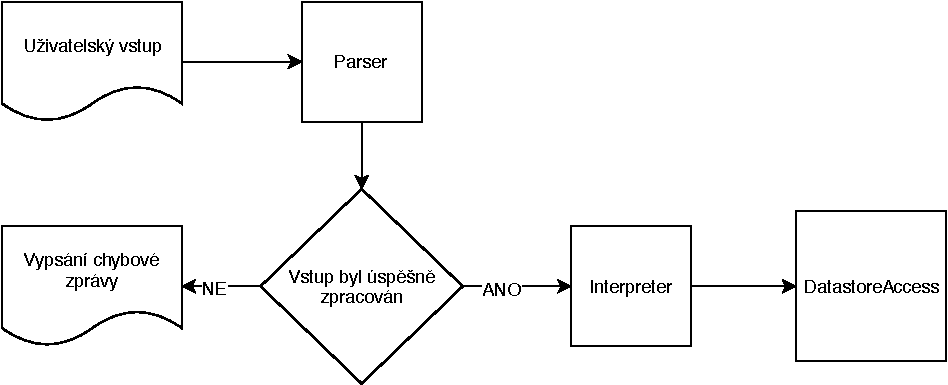
\includegraphics[width=.9\textwidth]{diagram}
\end{center}
\caption{Diagram proudu dat v programu}\label{proud:dat}
\end{figure}

\section{Uživatelské rozhraní}
Uživatelské rozhraní je poměrně přímočaré: program cyklicky načítá řádky uživatelského vstupu a zpracovává je. K interaktivnímu používání aplikace, je nutné implementovat nějaký způsob editace příkazové řádky. To zahrnuje především:
\begin{itemize}
    \item možnost úpravy aktuálního obsahu příkazové řádky před odesláním
    \item klávesové zkratky
    \item automatické doplňování příkazů
    \item ukládání historie příkazů
\end{itemize}
Ideální knihovna by měla mít nativní \Cpp{} rozhraní (ačkoliv lze v \Cpp{} relativně jednoduše použít i C knihovny) a být header-only, tedy, že k jejímu použití stačí přidat její hlavičkový soubor a všechny implementační detaily jsou obsaženy v něm.

Nejznámější knihovna využívaná k tomuto účelu je \textit{GNU Readline}\,\cite{readline}. \textit{Readline} umožňuje editaci příkazové řádky pomocí mnoha klávesových zkratek, převzatých z textových editorů \textit{EMACS} a \textit{Vi} a také velmi intuitivní inkrementální automatické doplňování (tj.\ postupné doplňování vícenásobným stisknutím klávesové zkratky). Nicméně, vzhledem k tomu, že je již poměrně zastaralá, má pouze rozhraní v jazyce C, tudíž to není dobrá volba pro moji aplikaci. Další nevýhodou je její implementace: \textit{Readline} obsahuje přibližně 20 tisíc řádek kódu především kvůli kompatibilitě s mnoha emulátory terminálů. V dnešní době většina terminálových aplikací podporuje základní VT100\footnote{druh terminálu} escape sekvence\footnote{kontrolní znaky, které slouží k ovládání terminálu; například mazání znaků nebo pohyb kurzorem} a tudíž není třeba zastaralé terminály podporovat.\cite{linenoise-readme}

Méně těžkotonážní variantou je knihovna \textit{linenoise}. Ta je oproti \textit{Readline} z hlediska velikosti zdrojového kódu velmi malá -- obsahuje zhruba tisíc řádků. Její odnož \textit{cpp-linenoise} je napsaná přímo v \Cpp{}, tudíž odpadají různé nevýhody použití jazyka C, a je header-only. Z hlediska funkčních požadavků \textit{cpp-linenoise} bohužel zaostává: nepodporuje mnoho klávesových zkratek (například kombinace klávesy Ctrl a směrových šipek) a automatické doplňování je pouze velmi jednoduché (neinkrementální). Všechny tyto nedostatky řeší knihovna \textit{replxx}. Ta oproti \textit{linenoise} není header-only, nicméně velmi dobře napodobuje \textit{Readline} z hlediska podpory klávesových zkratek a automatického dokončování. Ve svém programu jsem tedy zvolil knihovnu \textit{replxx}.

% TODO: ukázat docopt.cpp (Ale někde jinde)

\section{Zpracování vstupu pomocí \textit{Boost Spirit X3}}
Ke zpracování gramatik příkazů je potřeba parser.\footnote{syntaktický analyzátor; v mém programu část, která převádí textový vstup na strojově čitelný výstup} Implementaci parseru lze provést manuálně, to ovšem může být u složitých gramatik velmi nepraktické, a proto je vhodné použít nějakou knihovnu, která dokáže parser vygenerovat. Na základě konzultace s kolegou jsem použil knihovnu \textit{Boost Spirit X3}.

\subsection{\textit{Boost Spirit X3}}\todo{Možná nadpisy bez textit? YANG nadpis to třeba nemá}
\textit{Boost Spirit X3} je knihovna určená k vytváření parserů v jazyce \Cpp{}. Je součástí sady knihoven \textit{Boost}. Jednou z hlavních výhod \textit{Spiritu} je, že lze gramatiky zadávat přímo do zdrojového kódu výhradně pomocí prostředků jazyka -- operátorů\footnote{například plus, minus apod.} a \Cpp{} šablon. \Cpp{} umožňuje operátory předefinovat a tím změnit jejich funkcionalitu takřka libovolně. Důsledkem tohoto je, že není potřeba spouštět žádný preprocesor\footnote{program, který transformuje zdrojový kód před jeho vlastním zpracováním}, který by převedl speciální syntaxi parseru do validního \Cpp{} kódu. V následujících kapitolách vysvětlím, jakým způsobem lze \textit{Spirit} používat.

\subsection{Základní pravidla}
\textit{Spirit} generuje parsery pomocí pravidel. Základními stavebními bloky jsou pravidla pro terminály. Příkladem může být pravidlo \verb¨int_¨, které parsuje jedno celé číslo, nebo \verb¨char_¨, které parsuje právě jeden znak. Kromě těchto pravidel, \textit{Spirit} definuje i složitější elementární pravidla jako třeba \texttt{alpha}, které slouží k parsování znaků abecedy nebo \texttt{digit}, které parsuje číslici. K parsování právě jedno druhu znaku lze použít zápis znaku v \Cpp{} (například \verb¨'a'¨).

\subsection{Operátory}
Ke skládání pravidel ve \textit{Spiritu} slouží \Cpp{} operátory. Operátory lze různě kombinovat a zároveň funguje změna precedence operátorů pomocí závorek. Nyní popíšu funkci těch operátorů, které se v práci vyskytují.
\begin{description}
    \item[operátor \texttt{>>}]{Sekvence. \verb¨char_ >> char_¨ parsuje dva znaky za sebou. V EBNF se zapisuje pomocí čárky (\texttt{,}).}
    \item[operátor \texttt{*}]{\verb¨*char_¨ parsuje jakýkoliv znak nula až nekonečně krát. V EBNF se pravidlo obaluje složenými závorkami.}
    \item[operátor \texttt{+}]{\verb¨+char_¨ parsuje jakýkoliv znak jednou až nekonečně krát. V EBNF neexistuje.}
    \item[operátor \texttt{prefixové -}]{\verb¨-char_¨ parsuje jakýkoliv znak jednou nebo nula krát. V EBNF neexistuje.}
    \item[operátor \texttt{infixové -}]{\verb¨char_-'a'¨ parsuje jakýkoliv znak kromě znaku \uv{a}. V EBNF se zapisuje stejně.}
    \item[operátor \texttt{|}]{Alternativa. \verb¨char_ | int_¨ parsuje jakýkoliv znak nebo číslo. V EBNF se zapisuje stejně.}
\end{description}

\subsection{Definice pravidel ve \textit{Spiritu}}
Definovat pravidla lze dvěma způsoby. Jeden z nich je pomocí tzv.\ \texttt{auto} pravidel \texttt{auto} pravidla využívají \textit{type inference}, což je funkce \Cpp{}, která automaticky zjistí, o jaký typ proměnné se jedná a uživatel ho nemusí zadávat manuálně. Například deklarace \verb¨auto a = 0;¨ automaticky vyhodnotí, že datový typ proměnně \texttt{a} by měl být \texttt{int}. Vzhledem k tomu, že datový typ pravidel je takřka nemožné určit manuálně (název datového typu složitějších pravidel může mít kvůli šablonám i tísice znaků), je tedy klíčové slovo \texttt{auto} téměř nezbytné. \texttt{auto} pravidla lze vidět na ukázkách~\ref{spirit:grammar}~a~\ref{spirit:nonterminals}. Pro jednoduché parsery často \texttt{auto} pravidla stačí. Pro složitější parsery je třeba použít pokročilou formu definice pravidel, o které se zmiňuji v kapitole~\ref{advanced:rules}.

\subsection{Srovnání zápisu v EBNF a ve \textit{Spiritu}}
K zápisu gramatik používá \textit{Spirit} syntaxi, která se podobá syntaxi EBNF.\footnote{Extended Backus--Naur form} Rozdíl spočívá především v operátorech, které nemají v \Cpp{} postfixovou variantu, jako například operátor plus (\texttt{+}) nebo operátor násobení (\texttt{*}). V těchto případech je použita prefixová varianta operátoru. V ukázce~\ref{ebnf} je vidět EBNF gramatika, která odpovídá dvěma řetězcům, které jsou obalené uvozovkami.

\begin{listing}
\begin{verbatim}
not-a-quote = ... (* všechny znaky kromě uvozovky *)
quotedValue = '"' , not-a-quote , {not-a-quote} , '"'
twoQuotedValues = quotedValue , quotedValue
\end{verbatim}
\caption{Příklad EBNF}\label{ebnf}
\end{listing}

Na ukázce~\ref{spirit:grammar} je možné vidět způsob, jakým by se zapsala gramatika z ukázky~\ref{ebnf} ve \textit{Spiritu}. Samotné pravidlo \verb¨'"'¨ řiká, že pravidlo nejprve parsuje jednu uvozovku. Operátor \verb¨>>¨ značí sekvenci pravidel za sebou. \verb¨char:-'"'¨ znamená, že chceme parsenout jakýkoliv znak kromě uvozovky, a celé toto pravidlo je ještě obaleno operátorem \verb¨+¨, který celé vnitřní pravidlo zopakuje jednou až nekonečně krát (EBNF podporuje pouze nula až nekonečně krát). Na konci zbývá už jen pravidlo, které opět parsuje jednu uvozovku. Ve \textit{Spiritu} je každé takové pravidlo zároveň novým neterminálem a lze jej používat v jiných pravidlech stejně jako v EBNF\@. Gramatika v ukázce~\ref{spirit:nonterminals} parsuje právě dva uvozené řetězce, tak jak udává pravidlo \texttt{quotedValue}.

\begin{listing}
\begin{minted}{c++}
auto const quotedValue = '"' >> +(char_-'"') >> '"';
\end{minted}
\caption{Příklad gramatiky napsané ve \textit{Spiritu}}\label{spirit:grammar}
\end{listing}

\begin{listing}
\begin{minted}{c++}
auto const twoQuotedValues = quotedValue >> quotedValue;
\end{minted}
\caption{Skládání gramatik ve \textit{Spiritu}}\label{spirit:nonterminals}
\end{listing}


\subsection{Ukládání dat}
Abychom mohli pracovat s daty, které parser získá, je třeba je uložit do proměnných. K tomu ve \textit{Spiritu} slouží tzv.\ atributy pravidel. Atribut si lze představit jako datový typ návratových hodnot funkcí. Každé pravidlo má buď atribut \texttt{unused} (nevrací\footnote{\uv{vracením} je myšleno jaký atribut pravidlo vystavuje} nic), anebo některý z datových typů jazyka \Cpp{}. Příkladem může být jednoduché pravidlo \verb¨int_¨, které parsuje celé číslo a jeho atribut je datový typ \texttt{int}.

Pravidla ovšem nemusí vracet pouze primitivní datové typy, ale také celé datové struktury. Například pravidlo \verb¨+(char_-'"')¨ v ukázce~\ref{spirit:grammar} odpovídá řetězci (jednomu až mnoha znakům za sebou), a pro řetězce \textit{Spirit} určí datový typ \texttt{std::string}. Pravidlo v druhé ukázce~\ref{spirit:nonterminals} odpovídá parsování dovu řetězců za sebou. V tomto případě již \textit{Spirit} neumí odhadnout, jaký návratový typ očekáváme, a musíme ho zadat manuálně. V našem případě chceme uložit oba dva řetězce do dvou různých proměnných a ty sdružíme do \Cpp{} struktury, kterou můžeme vidět na ukázce~\ref{spirit:struct}. Tato struktura je s pravidlem kombatibilní, tzn.\ lze do ní uložit návratovou hodnotu tohoto pravidla.

\begin{listing}
\begin{minted}{c++}
struct TwoStrings {
    std::string firstString;
    std::string secondString;
}
\end{minted}
\caption{Kompatibilní struktura}\label{spirit:struct}
\end{listing}

\subsection{Pokročilá definice pravidel}\label{advanced:rules}
Pokud chceme kromě gramatiky pravidel nastavit i nějaké další parametry, \texttt{auto} pravidla už nestačí. V ukázce~\ref{spirit:advancedrule} je ukázán příklad kompletní definice pravidla. Nejprve definujeme proměnnou typu \texttt{x3::rule}, kterou se budeme na pravidlo odkazovat. První parametr šablony (\texttt{MyClass}) používá \textit{Spirit} iterně k rozlišení pravidel a také slouží k definování různých vedlejších efektů, o kterých píšu v kapitole~\ref{sideeffects}. Druhý parametr šablony slouží k deklaraci atributu pravidla \texttt{TwoStrings}. Dále je třeba definovat gramatiku pravidla. To se dělá pomocí \textit{auto} pravidel, jejichž název končí na \verb¨:def¨. Nakonec je třeba ještě říct \textit{Spiritu} o pravidlu pomocí makra \verb¨BOOST_SPIRIT_DEFINE¨.

\begin{listing}
\begin{minted}{c++}
x3::rule<MyClass, TwoStrings> const twoQuotedValues;

auto const quotedValue = '"' >> +(char_-'"') >> '"';
auto const twoQuotedValues_def = quotedValue >> quotedValue;

BOOST_SPIRIT_DEFINE(twoStrings)
\end{minted}
\caption{Pokročilá definice pravidla}\label{spirit:advancedrule}
\end{listing}

\subsection{Vedlejší efekty pravidel}\label{sideeffects}
Ačkoliv lze pomocí \textit{Spiritu} zapsat poměrně složité parsery, ne vždy může být jednoduché vytvořit gramatiku, která by ho generovala. Kvůli tomu \textit{Spirit} umožňuje na určitá místa vkládat kromě deklarativního\footnote{deklarativní kód je kód, kde programátor definuje, co má program udělat, ale ne jakým způsobem; to jsou například gramatiky ve \textit{Spiritu}} kódu i kód imperativní.\footnote{imperativní kód je kód, kde progrmátor určuje přesný postup algoritmu} Jedním ze způsobů, jak přidat imperativní kód je pomocí \uv{sémantických funkcí}. Pomocí operátoru hranaté závorky (\verb¨[]¨) je možné k pravidlu přiřadit volatelný objekt (funkci, lambda funkci nebo funktor) a po úspěšném parsenutí pravidla se objekt zavolá. V ukázce~\ref{spirit:semantic} lze vidět příklad použití. Pokud pravidlo úspěšně parsene číslo, program vypíše \uv{Hello, world!}.

\begin{listing}
\begin{minted}{c++}
auto const greeting = [] {
    std::cout << "Hello, world!" << std::endl;
};
auto const rule = int_[greeting];
\end{minted}
\caption{Sémantické akce}\label{spirit:semantic}
\end{listing}

Nevýhodou sémantických akcí je, že jejich používání velmi znepřehledňuje kód gramatik. Z tohoto důvodu existuje druhý způsob, jak přiřadit pravidlům imperativní kód a to pomocí \verb¨on_success¨ procedur. Zde hraje roli první parametr šablony \texttt{x3::rule}. Pokud do třídy, kterou v parametru uvedeme, nadefinujeme metodu \verb¨on_success¨, tato metoda se zavolá pří úspěšném parsenutí pravidla podobným způsobem jako fungují sémantické akce. Výhodou je, že tímto způsobem oddělíme gramatiky od imperativního kódu a gramatiky se stanou čitelnějšími.

V ukázce~\ref{spirit:handler} můžeme vidět příklad jak zapsat třídu s \verb¨on_success¨ metodou. V této metodě máme k dispozici čtyři parametry, které poksytují informace o stavu parseru a také možnosti jak chování parseru ovlivnit:
\begin{description}
    \item[begin]{iterátor, který ukazuje, kde parsování začalo}
    \item[end]{iterátor, který ukazuje, kde parsování skončilo}
    \item[ast]{reference na atribut, které pravidlo vrací}
    \item[context]{parametr, pomocí kterého lze ovládat chování parseru}
\end{description}

\begin{listing}
\begin{minted}{c++}
struct greeting {
    template <typename T, typename Iterator, typename Context>
    inline void on_success(Iterator const& begin,
                           Iterator const& end,
                           T& ast,
                           Context const& context)
    {
        std::cout << "Hello, world!" << std::endl;
    }
}

x3::rule<greeting, int> const rule;

auto const rule_def = int_;
BOOST_SPIRIT_DEFINE(rule)
\end{minted}
\caption{Metoda \texttt{on\_success}}\label{spirit:handler}
\end{listing}

\section{Implementace syntaxe}
V následujících kapitolách se zabývám způsoby implementace syntaxe, která je popsána v kapitole~\ref{syntaxe}.


\subsection{Příkazy}
Vytvořit gramatiky samotných příkazů podle jejich syntaxe je poměrně jednoduché. Nejsložitější gramatiku má příkaz \texttt{ls}, kterou lze vidět v ukázce~\ref{grammar:ls}. Nejprve gramatika parsuje řetězec \verb¨"ls"¨ (uložený v proměnné \verb¨ls:::name¨). Nyní je potřeba parsenout volitelný přepínač \verb¨ls_options¨. Samotné pravidlo pro tento přepínač je uvedeno v ukázce~\ref{grammar:ls:options}. Toto pravidlo je implementováno pomocí \uv{symbol table}, což je způsob, jak definovat, které řetězce se mají parsenout a jaké atributy budou mít.

\begin{listing}
\begin{minted}{c++}
auto const ls_def =
    ls_::name >> *(space_separator >> ls_options)
    >> -(space_separator >> (dataPathListEnd |
                             dataPath |
                             schemaPath));
\end{minted}
\caption{Gramatika příkazu \texttt{ls}}\label{grammar:ls}
\end{listing}


\begin{listing}
\begin{minted}{c++}
struct ls_options_table : x3::symbols<LsOption> {
    ls_options_table()
    {
    add
        ("--recursive", LsOption::Recursive);
    }
} const ls_options;
\end{minted}
\caption{Pravidlo \texttt{ls\_options}}\label{grammar:ls:options}
\end{listing}

Dále je nutné zajistit, aby program vyžadoval mezery mezi jednotlivýmy fragmenty příkazu. To zajišťuje pravidlo \verb¨space_separator¨, které je možné vidět na ukázce~\ref{grammar:space:separator}. Důvodem, proč je pravidlo poněkud složitější, je, že způsob, jakým v programu parsuju příkazy automaticky přeskakuje mezery. Tomu lze manuálně zábranit direktivou \verb¨x3::no_skip¨. Direktivy obalují pravidla a mění jejich vlastnosti, v tomto případě vypnutí přeskakování mezer. Druhou použitou direktivou je \verb¨x3::omit¨, která způsobí, že se zahodí atribut pravidla.

\begin{listing}
\begin{minted}{c++}
auto const space_separator =
    x3::omit[x3::no_skip[space]];
\end{minted}
\caption{Pravidlo \texttt{ls\_options}}\label{grammar:ls:options}
\end{listing}

Nakonec je třeba zapsat gramatiku pro argument cesty. Vzhledem k tomu, že \texttt{ls} přijímá jakoukoli cestu, v gramatice jsou jako alternativy vypsány všechny druhy cest. O implementaci pravidla pro cesty mluvím v následující kapitole.

\subsection{Cesty}
Implementace syntaxe pro cesty je nejsložitější gramatikou z celého programu. Důvodem je to, že názvy uzlů v cestě se mění na základě modelů \textit{YANG} a program je musí kontrolovat dynamicky. Vzhledem k tomu, že pravidla jsou pevně daná a neexistuje mnoho prostředků pro vytváření dynamických pravidel, rozhodl jsem se provést kontrolu názvů uzlů pomocí imperativního kódu, který zakomponuji do \verb¨on_success¨ metod jednotlivých pravidel.

Nejprve ale k samotným gramatikám. Gramatika pro schematickou cestu cestu vypadá takto:
\begin{minted}{c++}
auto const schemaPath_def =
    initializePath >> absoluteStart >> createPathSuggestions >>
    x3::attr(decltype(schemaPath_::m_nodes)()) >>
    x3::attr(TrailingSlash::NonPresent) >> x3::eoi
    |
    initializePath >> -(absoluteStart >> createPathSuggestions) >>
    schemaNode % '/' >> (trailingSlash >> createPathSuggestions >>
    (completing | x3::eoi) | (&space_separator | x3::eoi));

\end{minted}
Celé pravidlo pro schematickou cestu je rozdělené do dvou větví (pomocí operátoru \texttt{|}). První větev odpovídá samotnému lomítku -- tedy, když chce uživatel zadat jako cestu kořen stromu. Druhá větev odpovídá cestě, v které je alespoň jeden uzel.

Hlavní částí první větve je pravidlo \texttt{absoluteStart}. Je velmi jednoduché -- parsuje lomítko a jeho atribut je příznak, který řiká, že uživatel zadal absolutní cestu.\footnote{z hlediska \uv{absolutnosti} je cesta, která obsahuje pouze lomítko absolutní} Druhé pravidlo, které je zde důležité je \texttt{x3::eoi}. To způsobuje, že větev bude platná pouze pokud uživatel lomítko a žádný vstup navíc. Pravidla \texttt{x3::attr} zajišťují, že obě větve budou kompatibilní co se týče atributů.

Druhá větev parsuje názvy uzlů pomocí pravidla \verb¨schemaNode % '/'¨. Operátor procento (\texttt{\%}) aplikované na pravidlo způsobuje, že se parsene seznam položek oddělených znakem, který je na pravé straně od procenta. V tomto případě se tedy parsuje několik řetězců, které podléhají pravidlu \texttt{schemaNode} a které jsou odděleny lomítkem. To odpovídá stanovené syntaxi cest. Zbylá pravidla jsou pouze \uv{pseudopravidla}. Jejich gramatiky nic neparsují\footnote{obsahují pouze \texttt{x3::eps}, neboli epsilon} a slouží pouze k zavolání imperativního kódu. Pomocí těchto pravidel je také implementováno automatické doplňování, o kterém mluvim v kapitole~\ref{completion}.

Pravidlo \texttt{schemaNode} parsuje jednotlivé názvy uzlů. Jeho gramatika vypadá takto:
\begin{minted}{c++}
auto const schemaNode_def =
createPathSuggestions >> -(module) >> (container |
                                       list |
                                       nodeup |
                                       leaf);
\end{minted}
Zde lze již vidět některé konstrukty \textit{YANG}. Za pravidly \texttt{container}, \texttt{list} a \texttt{leaf} se skrývají gramatiky, které určují platný název uzly v modelu \texttt{YANG}. Liší se především v jejich \verb¨on_success¨ metodách. V těchto metodách je probíhá zmiňovaná dynamická kontrola názvů (a druhů) uzlů. V následujících podkapitolách popisuji jakým je tato kontrola implementována.

\subsubsection{Rozhraní \texttt{Schema}}
Ke kontrole cest slouží abstraktní rozhraní \texttt{Schema}. Toto rozhraní obsahuje různé metody pro kontrolu cest jako například \texttt{isLeaf}, která zjišťuje, jestli je uzel s danou cestou uzel typu \texttt{leaf}. Konkrétně je toto rozhraní implementováno jako třída \texttt{StaticSchema}, která je určená k testování, a jako třída \texttt{YangSchema}, která využívá knihovnu \textit{libyang}~\cite{libyang}. \textit{Libyang} je knihovna vytvořená spoečností CESNET, která umožňuje manipulovat s modely \textit{YANG}.

\subsubsection{Kontrola cest}
Kontrola cest probíhá v \verb¨on_success¨ metodách pravidel pro jednotlivé typy uzlů. Pomocí direktivy \texttt{x3::with} umožňuje \textit{Spirit} vložit do gramatiky jakýkoliv objekt, který lze poté v těchto metodách použít. Pro kontrolu cest by stačilo do startovacího pravidla\footnote{pravidlo, kde jsou sdruženy pravidlo pro všechny příkazy} vložit objekt typu \texttt{Schema}, nicméně je třeba, aby parser propagoval i nějaké další informace (kromě samotných příkazů) zpět. Proto jsem vytvořil třídy \texttt{ParserContext}, která obsahuje mimojiné několik proměnných, které jsou potřebné pro validaci cest. Jedna z nich je rozhraní \texttt{Schema} a další je akuální uzel, v kterém se parser nachází.

Implementace metod je poté poměrně jednoduchá -- v závislosti na typu uzlu se zavolá příslušná metoda (např.\ \texttt{isLeaf}) rozhraní Schema. Pokud rozhraní vrátí pozitivní odpověď, je název uzlu přijat a parsování pokračuje. Pokud bude odpověď negativní je třeba parser zastavit. Ukázka~\ref{on:success} ukazuje, jak vypadá \verb¨on:success¨ metoda pro \texttt{leaf}. Nejprve metoda získá pomocí \texttt{x3::get} vloženou instanci \texttt{ParserContext}, poté zavolá metodu \texttt{isLeaf} s aktuálním uzlem a na základě výsledku může parseru říct, že pravidlo ve skutečnosti proběhlo úspěšně (pomocí \verb¨_pass(context) = false;¨).

\begin{listing}
\begin{minted}{c++}
struct leaf_class {
    template <typename T, typename Iterator, typename Context>
    void on_success(Iterator const&, Iterator const&, T& ast, Context const& context)
    {
        auto& parserContext = x3::get<parser_context_tag>(context);
        const auto& schema = parserContext.m_schema;

        if (!schema.isLeaf(parserContext.m_curPath,
                           {parserContext.m_curModule, ast.m_name}))
            _pass(context) = false;
    }
};
\end{minted}
\caption{\texttt{on\_success} metoda pro \texttt{leaf}}
\end{listing}


\subsection{Automatické doplňování}\label{completion}

\section{Interpreter}
Další součástí programu je interpreter. Vzhledem k tomu, že je \textit{Spirit} schopen získat příkazy od uživatele v podobně velmi dobře čitelné strojem, není složité podle nich implementovat správnou funkcionalitu. Práce interpreteru je v zásadě jen volání správných procedur třídy \texttt{DatastoreAccess}.

\section{DatastoreAccess}
\subsection{Přístup k úložišti konfigurace}
K vykonávání příkazů potřebuje interpreter přístup k datovému úložišti. Toto je implementováno pomocí abstraktního rozhraní \texttt{DatastoreAccess}. Tato součást obsahuje procedury k nastavování leafů na různé hodnoty a jiné metody na změnu konfigurace. V mé aplikaci budou implementována tato konkrétní rozhraní:

\subsection{NetconfAccess}
% TODO: ukázat libnetconf2

\subsubsection{SysrepoAccess}
% TODO: ukázat sysrepo klientskou knihovnu

\section{Testování}
% TODO: ukázat doctest
% TODO: ukázat trompeloeil
% TODO: zmínit Catch

\subsection{Knihovna na logování?}
% TODO: spdlog, použito jen v netconf cpp wrapperu... od Honzy


\chapter{Vyhodnocení}
\section{Testování}
% TODO: testování přes doctest, především unit testy, ale i nějaký jiný (sysrepo.cpp)\@. hlášení bugů přes issue tracker, po opravení napsán test
\section{Porovnání s konkurencí}
% TODO: popsat, že ačkoliv moje aplikace nepodporuje 100 \% YANGu/NETCONFu, na základní použití stačí (hlavní cíl byl, upravovat konfiguraci bez znalosti YANG modelů a NETCONFu)
\section{Výsledky z nasazení}
% TODO: no, prej to Honza používá xD

\begin{conclusion}
% TODO: Něco dopsat sem, asi v závislosti na zbytku
\end{conclusion}

\printbibliography{}

\appendix

\chapter{Seznam použitých zkratek}
% \printglossaries
\begin{description}
    \item[GUI] Graphical user interface
    \item[XML] Extensible markup language
\end{description}

\chapter{Obsah přiloženého CD}

%\begin{figure}
%	\dirtree{
%            .1
%	}
%\end{figure}

\end{document}
